%-*- coding: utf-8 -*-
\subsection{Renseigner profil patient}

L'analyse du cas d'utilisation renseigner un profil pâtient se fait en plusieurs opérations : l'ajout, la modification, suppression et la validation de profil patient, qui sont implémentées selon un modèle MVC.

\begin{figure}
  \label{diagramme-renseigner-les-profils-patients}
  \centering
  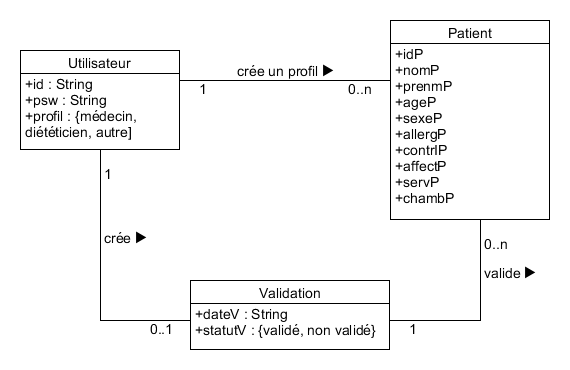
\includegraphics[width=0.9\textwidth]{../../CasDUtilisations/ProfilPatient/diagclassProfilPatient.png}
  \caption{Diagramme de classe renseigner les profils patients}
\end{figure}


\begin{figure}
  \label{diagramme-renseigner-les-profils-patients}
  \centering
  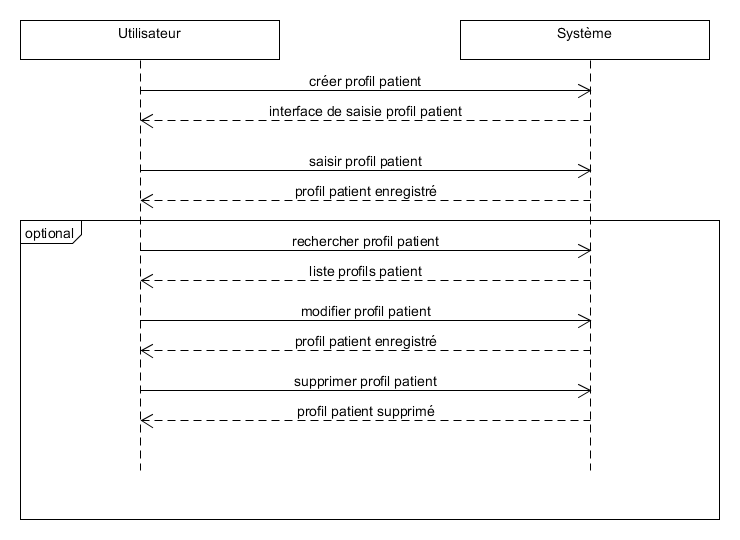
\includegraphics[width=0.9\textwidth]{../../CasDUtilisations/ProfilPatient/diagseqProfilPatient.png}
  \caption{Diagramme de séquence renseigner les profils patients}
\end{figure}

\begin{figure}
  \label{diagramme-renseigner-les-profils-patients}
  \centering
  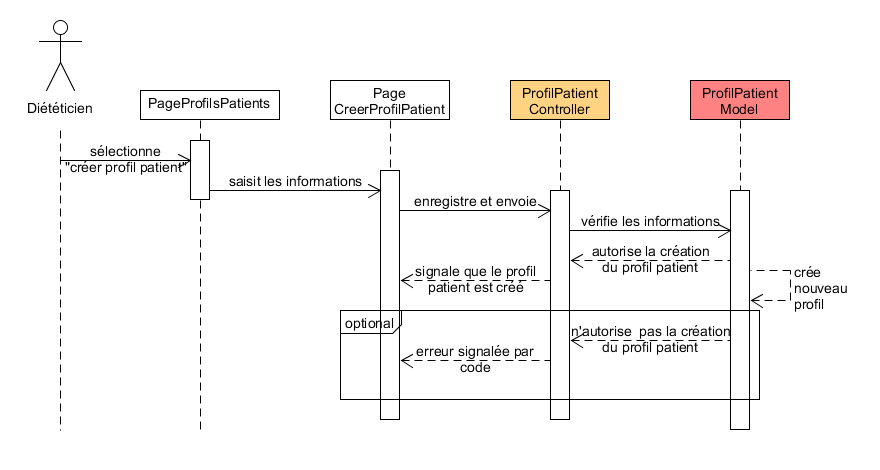
\includegraphics[width=0.9\textwidth]{../../CasDUtilisations/ProfilPatient/diagSrqDetaillProfilPatient.png}
  \caption{Diagramme de séquence détaillé renseigner les profils patients}
\end{figure}

\begin{figure}
  \label{diagramme-renseigner-les-profils-patients}
  \centering
  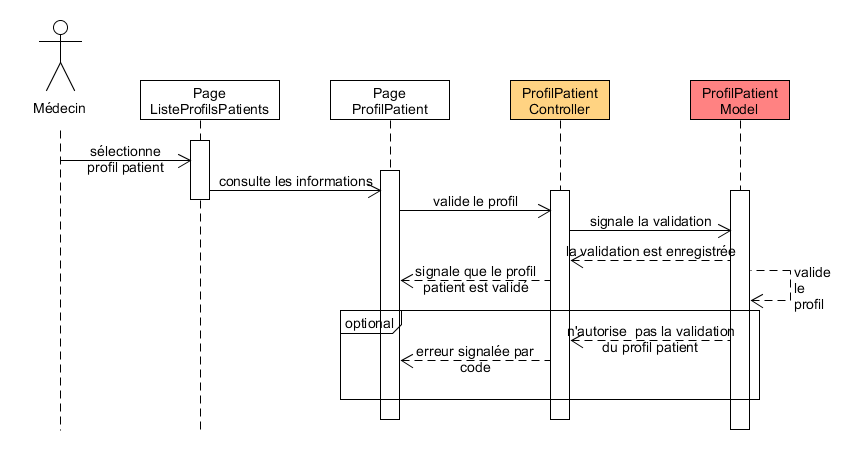
\includegraphics[width=0.9\textwidth]{../../CasDUtilisations/ProfilPatient/diagSrqDetaillValidProfilPatient.png}
  \caption{Diagramme de séquence détaillé valider les profils patients}
\end{figure}
